%% Supplementary Information accompanying article_cac.tex.
%% Standalone document; source provenance and limitations are in Note 6.
\documentclass[11pt]{article}
\usepackage[margin=2.4cm]{geometry}
\usepackage{graphicx}
\usepackage{amsmath,amssymb}
\usepackage{booktabs}
\usepackage{array}
\usepackage{multirow}
\usepackage{adjustbox}
\usepackage{parskip}
\usepackage{xcolor}
\usepackage[colorlinks=true,allcolors=blue]{hyperref}
\setlength{\parindent}{0pt}

\renewcommand{\thefigure}{S\arabic{figure}}
\renewcommand{\thetable}{S\arabic{table}}

\title{Supplementary Information\\[4pt]
\large Characterizing and mitigating the in-context cliff:
a complementary learning systems perspective on fast and slow learning in large language models}
\author{Anonymous}
\date{}

\begin{document}
\maketitle

\tableofcontents
\bigskip
\hrule

% =====================================================================
\section*{Supplementary Note 1: prompt template and evaluation}
\addcontentsline{toc}{section}{Note 1: prompt template and evaluation}
\label{snote:prompt}

The prompt concatenates a fixed task instruction, demonstrations drawn from a
\textcolor{blue}{disjoint} pool, and a single query, rendered with the model's native chat template.
\textcolor{blue}{The panel sampler uses} a per-class quota of
\textcolor{blue}{$\max(1,\lfloor K/C\rfloor)$} for a $C$-class task \textcolor{blue}{and then slices to requested} $K$\textcolor{blue}{.
With sufficient class supplies, at requested} $K{=}64$ this supplies 64 demonstrations for
four-class ag\_news, 63 for three-class MNLI and 60 for six-class trec\textcolor{blue}{; when $K<C$ it can
still return $K$ demonstrations, without class balance}. Within a
cell all queries share one demonstration draw. \textcolor{blue}{In the descriptive regional panel,
seed-to-seed spread is variability across demonstration draws; independent training
blocks in the controlled study are defined separately in Note~8.}

\textcolor{blue}{Recorded query counts vary: the selected Llama and Mistral regional runs use 200 queries
per draw, whereas DeepSeek and InternLM2.5 use 100 (Table}~\textcolor{blue}{\ref{stab:protocols}}\textcolor{blue}{); the
mechanistic run also uses 100.} Query sets are \textcolor{blue}{not necessarily class-balanced,} and \textcolor{blue}{exact
query identities, prompt lengths and common hosted decoding settings for the panel} are not
\textcolor{blue}{uniformly recorded}. Outputs are mapped to the label set by constrained string matching;
a response matching no label is counted \emph{unparseable} and scored as incorrect.
\textcolor{blue}{Total} accuracy \textcolor{blue}{includes these errors; accuracy conditional on valid labels uses} a \textcolor{blue}{selected
denominator. Neither parseability nor a parseable mistake identifies a} content\textcolor{blue}{-integration
mechanism} (Supplementary Note~4).

% =====================================================================
\section*{Supplementary Note 2: the fast path leaves no trace across prompts}
\addcontentsline{toc}{section}{Note 2: statelessness of the fast path}
\label{snote:stateless}

To summarize cross-prompt consistency, we evaluate a fixed query
set for task~A, run a $K{=}16$ in-context episode on a different task~B, then re-evaluate
the identical task-A query set. Backward transfer is the change in task-A accuracy between
the two evaluations. Across 50 task-pair/seed combinations the change lies within $-0.040$ to $+0.020$,
with a mean of $-0.003$\textcolor{blue}{; these aggregate differences do not establish persistent state.}

We stress that this outcome is expected \emph{by construction}: a frozen model carries no
state between forward passes, so no residue is possible. We report it because the mapping
in Table~1 of the main text asserts statelessness as a property of the fast path, and it
is \textcolor{blue}{a consistency check rather than} an empirical discovery\textcolor{blue}{. Identical deterministic inputs
would give identical outputs;} the \textcolor{blue}{aggregate differences do not establish a carry-over
effect or show} that \textcolor{blue}{weight learning is necessary for} durable \textcolor{blue}{adaptation.}

% =====================================================================
\section*{Supplementary Note 3: the synthetic\textcolor{blue}{-rule} probe was uninformative}
\addcontentsline{toc}{section}{Note 3: the synthetic-rule probe (negative result)}
\label{snote:synthetic}

Synthetic rule-classification tasks probe the distinction between in-context \emph{learning}
and in-context \emph{retrieval}, \textcolor{blue}{with rules intended to reduce direct benchmark
contamination}. Each task pairs a fixed vocabulary of surface tokens with an
arbitrary deterministic rule (for \texttt{rule\_v1}, a binary task: the label is
determined by whether the final word contains more than two vowels). \textcolor{blue}{The mapping is
intended to require inference from examples, but} above-chance accuracy
\textcolor{blue}{alone would not distinguish rule inference from other uses of prior knowledge.}

\textbf{The probe \textcolor{blue}{did not establish} the \textcolor{blue}{intended distinction.}} \textcolor{blue}{Some reported means exceed
$0.50$, including $0.572$ for Gemma-3-27B} at \textcolor{blue}{$K{=}64$} (Table~\ref{stab:synth})\textcolor{blue}{; we do not
claim that every result is at chance}. First, \textcolor{blue}{Llama-3.1-8B} scores
\emph{higher} than \textcolor{blue}{Gemma-3-4B} at every \textcolor{blue}{measured many-shot} $K$: Llama-3.1-8B sits at
$0.517$--$0.543$ while Gemma-3-4B sits at $0.480$--$0.512$, against a chance level of
$0.50$. Second, zero-shot accuracy \textcolor{blue}{in the separate sweep} is already
$0.440$--$0.547$, \textcolor{blue}{overlapping} many-shot values\textcolor{blue}{. These summaries do not supply a
validated within-pipeline learning-versus-retrieval test.}

We therefore draw no learning-versus-retrieval conclusion, and we note that a synthetic
probe on which at least one model demonstrably learns the rule is a prerequisite for
testing that distinction. We consider the most likely explanation to be that the rules are
too far outside the distribution of formats these models were aligned on to be learnable
from tens of examples, rather than that no model can bind novel input--label mappings; but
we have not established this, and the released task generators are provided so the
question can be revisited.

\begin{table}[h]
\centering
\caption{\textbf{Accuracy on the synthetic rule task
(\texttt{rule\_v1}, binary, chance $=0.50$).} Zero-shot values are from the separate
zero-shot sweep\textcolor{blue}{; they are not a paired treatment baseline. Natural-task regime tags refer
to the illustrated natural-task curves, not universal} model \textcolor{blue}{properties. The probe} does
not \textcolor{blue}{establish} the \textcolor{blue}{intended learning-versus-retrieval distinction}.
Values are means over 10 demonstration draws ($K{\geq}1$) and 3 draws ($K{=}0$).}
\label{stab:synth}
\footnotesize
\begin{tabular}{llccccc}
\toprule
Model & Regime & $K{=}0$ & $K{=}1$ & $K{=}4$ & $K{=}16$ & $K{=}64$ \\
\midrule
Llama-3.1-8B-Instruct & cliff-prone   & --      & 0.517 & 0.539 & 0.543 & 0.539 \\
DeepSeek-V3.2         & cliff-prone   & 0.440   & 0.505 & 0.535 & 0.510 & 0.525 \\
Gemma-3-4B-it         & cliff-immune  & 0.513   & 0.483 & 0.480 & 0.495 & 0.512 \\
Gemma-3-12B-it        & cliff-immune  & 0.547   & 0.487 & 0.521 & 0.533 & 0.519 \\
Gemma-3-27B-it        & cliff-immune  & 0.520   & 0.476 & 0.514 & 0.522 & 0.572 \\
Qwen3-32B             & cliff-immune  & 0.517   & 0.491 & 0.527 & 0.532 & 0.514 \\
Llama-3.3-70B-Instruct& cliff-immune  & 0.500   & 0.487 & 0.531 & 0.552 & 0.543 \\
\bottomrule
\end{tabular}
\end{table}

% =====================================================================
\section*{Supplementary Note 4: decode failures and how they are handled}
\addcontentsline{toc}{section}{Note 4: decode failures}
\label{snote:decode}

Because unparseable outputs are scored as incorrect, a cell in which the model emits no
matchable label at all registers \textcolor{blue}{total} accuracy $0.000$\textcolor{blue}{, with conditional valid-label
accuracy undefined. Across all reported before/after source paths, 299 of 3}{\textcolor{blue}{,}}\textcolor{blue}{222
query--draw cells have zero accuracy and $200/200$ unparseable outputs. Retaining one
copy per byte-identical file gives 281 of 2}{\textcolor{blue}{,}}\textcolor{blue}{958 cells; these are} not \textcolor{blue}{independent
training replicates. The corresponding directory-only counts for
\path{results/interventions/}} \textcolor{blue}{are} 265 of 3{,}102\textcolor{blue}{. These aggregate cells do not
identify whether a sequence-budget limit caused an individual failure. The controlled
study records input lengths and rejects overflowing prompts without truncation (Note~8).}

\textcolor{blue}{Under the nominal late-region fine-tuning on sst2 at $K{=}64$, all five evaluation draws
produced $200/200$ unparseable outputs. This is a decode failure, without an inference of
semantic destabilization. Table}~\textcolor{blue}{\ref{stab:region}} \textcolor{blue}{reports descriptive means and draw ranges;
no training-level Welch tests are reported because independent retraining is unverified.
Partial invalidity also matters: late trec total accuracy changes $0.302\to0.197$, while
invalid outputs increase $27/1{,}000\to446/1{,}000$. Pooled valid-label ratios are
$0.310\to0.356$ on denominators 973 and 554. The surviving subsets differ, so this
conditional comparison does not establish semantic improvement or impairment.}

% =====================================================================
\section*{Supplementary Note 5: intervention targeting, objective, and known caveats}
\addcontentsline{toc}{section}{Note 5: intervention caveats}
\label{snote:caveats}

\textcolor{blue}{The main regional conclusions use the exact-target, 18-adapter cohort in Note~9. The nominal regional, depth/component, transfer and self-target comparisons in this note and Tables~S5--S12 are retained as descriptive observations with incomplete original targeting provenance. They do not authenticate a regional causal ordering or replace the verified cohort. Differences in query panels, objectives and calibration budgets preclude pooling their means with the main table.}

Three properties of the intervention implementation bound the interpretation of the
\textcolor{blue}{regional fine-tuning} results\textcolor{blue}{.}

\textbf{\textcolor{blue}{Regional scope.}} \textcolor{blue}{Region and window labels in the descriptive
panel denote nominal block designs. These aggregate results do not authenticate exact
module membership or identify causal failure locations. The controlled study separately
verifies all 32 adapted attention projections in blocks 12--19 and their 3,407,872
trainable parameters (Note~8).}

\textbf{The objective is whole-prompt language modelling.} The calibration loss is
next-token prediction over the entire sequence, prompt and demonstrations included, not
over the label span alone. \textcolor{blue}{The label-only controls in Note~8 separate this objective
from supervision restricted to the query label. Regional gains measure adaptation
efficacy} rather than the \textcolor{blue}{original failure's location. We distinguish recovery
$R(K)=a_{\rm after}(K)-a_{\rm before}(K)$, zero-shot change $R(0)$} and
\textcolor{blue}{$S(K)=R(K)-R(0)$ (Table}~\textcolor{blue}{\ref{stab:components}}\textcolor{blue}{). Positive specificity alone} does not \textcolor{blue}{establish
zero-shot preservation; the nominal four-block attention example has $R(16)=+0.407$
and $R(0)=-0.165$.}

\textbf{\textcolor{blue}{Reverse-direction supervision audit.}} The \textcolor{blue}{selected}
reverse-direction supervision target is the label the model itself emits with no demonstrations.
When that zero-shot generation fails to parse, \texttt{\_k0\_prediction} falls back to the
first label in the task's label set (``World'' for ag\_news). A high fallback rate would
train the band toward a near-constant label and would supply an explanation for the observed
zero-shot decrement ($0.78\rightarrow0.45$) that does not require the early band to be
specifically implicated.

\textcolor{blue}{The audit evaluates a seeded} calibration \textcolor{blue}{draw} on the base model\textcolor{blue}{,} before \textcolor{blue}{an}
adapter is attached, and re-\textcolor{blue}{scores} zero-shot \textcolor{blue}{predictions} for 500 examples.
\textbf{The fallback fired 0 times in 500}
(Table~\ref{stab:fallback}). The targets are moreover well distributed across the four
classes, with a maximum class share of $36.8\%$ against a gold share of $27.2\%$, and they
agree with the gold label on $81.6\%$ of examples, consistent with this model's $0.78$--$0.785$
zero-shot accuracy on ag\_news. \textcolor{blue}{This audit addresses the fallback mechanism;
it does not authenticate the targets of every reverse protocol or
exclude other optimization,} calibration \textcolor{blue}{or precision effects.}

The \textcolor{blue}{selected early protocol changes ag\_}\textcolor{blue}{news zero-shot accuracy $0.78\to0.45$, with} a
\textcolor{blue}{$-0.018$ change at $K{=}16$;} the late \textcolor{blue}{zero-shot change is} $+0.025$\textcolor{blue}{, without an equivalence
test. The sst2 transfer result also shows collateral damage. This selected arm does not
confirm induction of a new many-shot cliff}, and \textcolor{blue}{all measured variants, including a
different nominal four-block Gemma candidate,} are \textcolor{blue}{retained (Note}~\textcolor{blue}{6)}. \textcolor{blue}{The recorded supervision audit is supplied as \path{results/interventions/induce_fallback_audit.json}, with its source identity in the complete inventory. The current reproduction entry point is \path{python -m publication.rebuild}; the original supervision audit remains a measured diagnostic rather than a new inference run.}
\textcolor{blue}{The audit records a SHA-256 of the target-construction source; its scope is
the measured supervision audit rather than authentication of every trained adapter.}

\begin{table}[h]
\centering
\caption{\textbf{\textcolor{blue}{Audit} of the \textcolor{blue}{selected} reverse-direction supervision target.} All 500 calibration examples
\textcolor{blue}{sampled with a fixed seed and scored} on the base Gemma-3-4B-it checkpoint. The
default-label fallback never fired, so the supervision signal is the model's own zero-shot
label throughout \textcolor{blue}{this audit; the result does not identify the targets of every reverse variant.}}
\label{stab:fallback}
\footnotesize
\begin{tabular}{lc}
\toprule
Quantity & Value \\
\midrule
Calibration examples                                   & 500 \\
Generations that parsed to a label                     & 500 (100.0\%) \\
Times the default-label fallback fired                 & \textbf{0 (0.0\%)} \\
Targets agreeing with the gold label                   & 408 (81.6\%) \\
Most common target class share (\emph{Business})       & 36.8\% \\
Most common gold class share (\emph{Business})          & 27.2\% \\
Target distribution (World / Sports / Business / Sci-Tech) & 134 / 120 / 184 / 62 \\
\bottomrule
\end{tabular}
\end{table}

\textbf{\textcolor{blue}{Precision and quantization.}} \textcolor{blue}{The controlled study and checkpoint/template
comparison use BF16 without quantization. Precision is not uniformly documented for the
descriptive panel, so the panel does not support an effect attributed to quantization or
a precision-matched comparison. Available per-cell settings are in the companion inventory.}

% =====================================================================
\section*{Supplementary Note 6: data provenance for every reported value}
\addcontentsline{toc}{section}{Note 6: data provenance}
\label{snote:prov}

\textcolor{blue}{Numerical summaries are derived within each source protocol;}
Table~\ref{stab:prov} maps each class to its source.
The behavioural panel and the \textcolor{blue}{regional fine-tuning} panel come from different pipelines with
slightly different zero-shot values for the same model and task (for Llama-3.1-8B on
ag\_news: $0.810$ hosted, $0.850$ self-hosted at $n{=}200$, $0.870$ in the mechanism run
at $n{=}100$). No quantity in the paper is computed by subtracting across pipelines, and
every before/after difference is within-run.

\begin{sloppypar}
\textcolor{blue}{The complete companion inventory covers 69 source paths and 63 distinct byte contents,
including 50 before/after paths with 45 distinct contents. Aliases are retained and counted
once in content-adjusted summaries; distinct contents are not assumed to be independent
training. The inventory records available model/band/calibration/task/draw metadata,
precision availability and nominal targeting, and use in the regional summaries.
The two nominal two-block versions give $R(16)=+0.585$ and $-0.040$; both are retained
without selecting by effect size. All 13 reverse paths (11 distinct contents) are likewise
retained, with full curves and the different four-block Gemma candidate described below. These aggregate comparisons are descriptive; independently trained
controlled adapters are reported separately in Note~8.
Companion files are \path{revision/generated/supplementary_run_inventory.csv}}\textcolor{blue}{,
\path{revision/generated/approved_regional_components.csv}}\textcolor{blue}{,
\path{revision/generated/approved_variant_protocols.csv}}\textcolor{blue}{,
\path{revision/generated/approved_variant_curves.csv}} \textcolor{blue}{and
\path{revision/generated/approved_full_curve_atlas.pdf}}\textcolor{blue}{. The complete dose/depth effect
table, including four-block and task-transfer protocols, is
\path{revision/generated/supplementary_dose_depth_effects.csv}}\textcolor{blue}{.}
\end{sloppypar}

\textcolor{blue}{The Qwen2.5-7B-Instruct no-cliff control uses five evaluation draws.
On AG News, nominal early-region training changes $K=16$ accuracy
$0.814\to0.844$, with $R(0)=+0.020$ and $S(16)=+0.010$; the late-region result
has $R(16)=0$, $R(0)=+0.045$ and $S(16)=-0.045$. This descriptive control
does not show a generic large early-region gain. Two induction-score comparison
protocols change Llama-3.1-8B $K=16$ accuracy $0.375\to0.825$ and
$0.4125\to0.9125$, while early/late induction scores change only $0.0011$--$0.0018$.
Thus recovery does not establish restoration of the measured induction score.}

\textcolor{blue}{The reverse-direction variants also constrain generality. Qwen2.5-1.5B
zero-shot AG News accuracy changes $0.755\to0.755$ (early), $0.675$ (middle)
and $0.785$ (late), with calibration $K=16$. For Qwen2.5-7B, calibration $K=8$
gives $0.790\to0.800$ (early) and $0.885$ (middle). Gemma-3-4B at calibration
$K=8$ changes $0.805\to0.840$ (middle) and $0.810$ (late). The large early
zero-shot decrement in the selected eight-block protocol is therefore observed in
one of three checkpoints, rather than a common reverse effect. A distinct nominal
four-block Gemma protocol raises zero-shot accuracy $0.790\to0.895$ while
lowering $K=16$ accuracy $0.825\to0.2967$; its different protocol and nominal
targeting do not provide a matched bidirectional causal test. The inventory retains
all variants and calibration tasks, including SST2/TREC depth and dose protocols.}

\begin{table}[h]
\centering
\caption{\textbf{Provenance of reported values.}}
\label{stab:prov}
\footnotesize
\setlength{\tabcolsep}{4pt}
\begin{adjustbox}{max width=\textwidth}
\begin{tabular}{@{}>{\raggedright\arraybackslash}p{0.25\textwidth}>{\raggedright\arraybackslash}p{0.56\textwidth}>{\raggedright\arraybackslash}p{0.14\textwidth}@{}}
\toprule
Claim class & Source & Pipeline \\
\midrule
Behavioural curves with $K{=}0$; recipe dissociation & \textcolor{blue}{\path{results/hosted_sweeps/recipe_difference_*.json}}\textcolor{blue}{, \path{hermes3_full.json}} & hosted API \\
DeepSeek-V3.2 and full-panel curves ($K{\geq}1$)     & \textcolor{blue}{\path{results/exp1a_complete.csv}} & hosted API \\
Synthetic-rule zero-shot                             & \textcolor{blue}{\path{results/exp1e_results.json}} & hosted API \\
Statelessness / backward transfer                    & \textcolor{blue}{\path{results/exp1b_results.json}} & hosted API \\
Region $\times$ task recovery                        & \textcolor{blue}{\path{results/interventions/remove_llama31_8b_*_results.json}}\textcolor{blue}{; exact rows in companion inventory} & self-hosted \\
Depth profile (4-block windows)                      & \textcolor{blue}{\path{results/interventions/remove_llama31_8b_blk*_n4_attn_results.json}} & self-hosted \\
Attention vs MLP component cut                       & \textcolor{blue}{\path{results/interventions/remove_llama31_8b_blk*_n4_*_results.json}}\textcolor{blue}{; selected attention/MLP rows in companion inventory} & self-hosted \\
Per-projection cut                                   & \textcolor{blue}{\path{results/component_dissociation.csv}} & self-hosted \\
Cross-\textcolor{blue}{checkpoint regional comparison}                 & \textcolor{blue}{\path{results/interventions/remove_*_results.json}}\textcolor{blue}{; selected rows in companion inventory} & self-hosted \\
Reverse-direction arm                                & \textcolor{blue}{\path{results/interventions/induce_*_results.json}}\textcolor{blue}{; all protocols retained} & self-hosted \\
Reverse-direction supervision audit                  & \textcolor{blue}{\path{results/interventions/induce_fallback_audit.json}} & self-hosted \\
\textcolor{blue}{Mean residual-state replacement}, induction \textcolor{blue}{scores}     & \textcolor{blue}{\path{results/interventions/t5_llama31_8b_ag_news_results.json}} & self-hosted \\
\textcolor{blue}{Controlled adaptation, readouts, curves, formats and transfer} & \textcolor{blue}{\path{revision/final_integration/supplement_table_sources.json}; Tables~\ref{stab:final_training}--\ref{stab:final_transfer}} & \textcolor{blue}{self-hosted BF16} \\
\bottomrule
\end{tabular}
\end{adjustbox}
\end{table}

\section*{\textcolor{blue}{Supplementary Note 7: demonstration bias and order controls}}
\addcontentsline{toc}{section}{Note 7: development bias and order controls}
\label{snote:w3}

\textcolor{blue}{Llama-3.1-8B-Instruct was evaluated on 100 AG News development queries, with three shared demonstration draws at $K{=}8,16,32$ and one shared zero-shot reference. Random, blocked, interleaved and class-assigned cyclic orders retain each demonstration multiset. Final-class assignments average two fixed last-example choices; these choices are not independent model or draw replicates. Majority-composition controls alter source examples despite length matching. The 29,200 design-query records include 28,900 distinct physical query prompts, with no truncation or rejection.}

\textcolor{blue}{Complete-label log likelihood $\ell_y(x)$ sums token log probabilities for a leading space and the full label, using a common conditioning prefix (and any boundary-retokenized prompt suffix), without length normalization. For the same demonstration context, each of the fixed content-free queries \texttt{N/A}, \texttt{[MASK]} and the empty string supplies a label-normalized probability vector. Their arithmetic mean is the prior $\pi_y$. Calibrated probabilities are
\[
 p_{\mathrm{cal}}(y\mid x)=\operatorname{softmax}_{y}\!\left[\ell_y(x)-\log\max(\pi_y,10^{-12})\right].
\]
Greedy generation remains a separate readout. The calibration comparison therefore pairs calibrated with raw likelihood, rather than comparing calibrated likelihood with generation. At $K{=}16$ in random order, the likelihood improvement is $+0.3933$ (pointwise 95\% query/draw bootstrap interval $[0.2233,0.5433]$); its zero-shot-adjusted change is $+0.4433$ $[0.2867,0.5900]$. Calibration mitigates this development decline but does not remove all high-$K$ loss: calibrated accuracy is $0.5867$ at $K{=}32$ versus $0.8100$ at $K{=}0$.}

\textcolor{blue}{Table~\ref{stab:w3} supplies selected descriptive results and the four final-class assignment contrasts. The intervals use 2,000 crossed query/draw resamples and average fixed context choices within query/draw cells. There are only three draw clusters, all order contrasts are exploratory and pointwise, and no multiplicity-adjusted or isolated final-token causal claim is made. The complete condition curves, label marginals, confusion matrices and paired contrasts are retained in \path{revision/generated/w3_condition_curves.csv}, \path{revision/generated/w3_label_marginals.csv}, \path{revision/generated/w3_confusions.csv} and \path{revision/generated/w3_paired_effects.csv}. The held-out calibration comparison uses a separate 200-query panel (Note~8); the order contrasts remain development analyses.}

\section*{\textcolor{blue}{Supplementary Note 8: controlled adaptation and held-out evaluations}}
\addcontentsline{toc}{section}{Note 8: controlled adaptation and held-out evaluations}
\label{snote:controlled}

\textcolor{blue}{On the 100-query AG News development panel, the earliest tested $K$ with
both an absolute decline of at least $0.10$ and a decline of at least $20\%$ relative
to the development peak is $K=16$. This fixes the controlled evaluation point;
the rule does not classify the multi-model panel and is not reapplied to select an
endpoint on the held-out 200-query results.}

\textcolor{blue}{A separate 500-query AG News behavioural panel confirms the native-template
decline in the untreated Llama-3.1-8B-Instruct checkpoint
(Table~\ref{stab:baseline500}). With five demonstration draws, accuracy is $83.00\%$
at zero shot and $38.20\%$ at $K=16$, a $44.80$-point decline with 95\% crossed
query/draw bootstrap interval $[34.92,55.12]$. The empirical majority baseline is
$28.60\%$. Only $24/18,000$ outputs across its full curve are invalid, with no
truncation or rejection. This behavioural confirmation cohort is separate from the
200-query controlled evaluation and the 100-query development analyses below.}

\textcolor{blue}{The controlled study fixes Llama-3.1-8B-Instruct, AG News and attention-only
LoRA in zero-based blocks 12--19 inclusive. All 32 query/key/value/output projections
are adapted (rank 16, $\alpha=32$; 3,407,872 trainable parameters). Each of three
independent calibration/training blocks samples 500 calibration queries and trains four
arms for two epochs, 250 optimizer updates, learning rate $2\times10^{-4}$ and gradient
accumulation four. Arm A uses eight correctly labelled demonstrations and whole-prompt
next-token loss. B uses the same contextual input with loss restricted to the gold query
label; C uses gold query-label loss without demonstrations. D uses contextual input
and shuffled query targets, preserving target-label marginals and allowing chance-correct
assignments; its demonstrations remain correctly labelled. B and C match query-label
presentations and optimizer updates, not input-token exposure. A supervises substantially
more tokens than the label-only arms. Calibration sampling and initialization vary
together across blocks, so their variance components are not separately identified.}

\textcolor{blue}{The primary evaluation shares 200 held-out AG News queries and five demonstration
draws at $K=16$ across all arms, with one zero-shot output per query and adapter.
Query, calibration, demonstration and technical-validation roles are disjoint by
recorded identity and text hash; the 200 queries also exclude the separate 500-query
behavioural confirmation panel. The primary panel's majority-class baseline is
$27.50\%$ (uniform-label chance $25.00\%$). Inference uses native chat formatting, BF16, greedy
generation and a ten-new-token cap. Overflowing prompts are rejected without
truncation. The complete-output parser accepts only a permitted label; additional
continuation is invalid and receives zero credit. Table~\ref{stab:final_training}
shows all twelve adapters and the shared untreated baseline, and
Table~\ref{stab:final_training_contrasts} reports paired effects. Pointwise 95\%
intervals use 2,000 crossed percentile bootstrap resamples of query identities,
demonstration draws and paired training blocks. Shared baseline predictions are not
independent training replicas. With only three training blocks and five draws,
interval coverage is limited; the analysis does not establish noninferiority,
familywise significance or population-wide preservation.}

\textcolor{blue}{B exceeds the demonstration-free task-learning control C at $K=16$ by
$39.17$ percentage points $[20.63,56.30]$, and the shuffled-target control D by
$64.80$ $[57.63,71.63]$. All three blocks favor B in both contrasts.
These results distinguish contextual adaptation from the matched zero-shot objective
in this setting, without localizing the original deficit. A reaches $89.37\%$ at
$K=16$ but has entirely invalid zero-shot output in all three blocks: it emits a
label followed by additional example text. We retain the strict zero-credit endpoint.
Complete-label likelihood gives A $88.17\%$ at $K=0$, demonstrating restricted-label
discrimination despite this output-format cost; it does not establish unconstrained
instruction following or general knowledge preservation (Table~\ref{stab:final_readouts}).}

\textcolor{blue}{Untreated generation concentrates on World at high $K$: $761/1,000$ outputs
at $K=16$ and $744/1,000$ at $K=32$, versus $50/200$ at zero shot. The gold World
share is $55/200$. Table~\ref{stab:final_confusions} gives the full confusion matrices;
the concentration supports examining label bias rather than inferring a unique
capacity mechanism from accuracy alone.}

\textcolor{blue}{The likelihood and content-free calibration definitions are those in Note~7,
with priors computed separately for the untreated model and each A adapter. On the
200-query panel, untreated calibrated likelihood is $73.30\%$ at $K=16$, versus
$30.70\%$ raw likelihood, a $42.60$-point gain $[33.40,51.50]$. Calibrated accuracy
is nevertheless below its $81.50\%$ zero-shot value, by $8.20$ points $[1.10,15.80]$;
at $K=32$ the deficit is $16.20$ $[6.90,24.20]$. Calibration therefore mitigates rather
than eliminates the decline. For A the primary calibrated-minus-raw contrast at
$K=16$ is $+0.20$ points $[-3.07,4.17]$; the distinct calibrated A-minus-untreated
contrast is $+16.27$ $[9.50,23.93]$. A positive between-model comparison does not
substitute for the within-model calibration contrast.}

\textcolor{blue}{Full curves for the untreated model and all three A adapters use a separate
100-query AG News development panel and three demonstration draws
(Table~\ref{stab:final_curves}). They show recovery at $K\geq8$, severe small-$K$
formatting costs, and between-block variation at larger $K$; they are not independent
primary confirmation or evidence of uniform repair. The checkpoint/template
comparison uses the same primary 200 queries, five draws and $K=0,16,32$
(Table~\ref{stab:final_formats}). Its neutral common format has identical text and
input token IDs across Instruct, Hermes-3 and their base checkpoint. Under the strict
generation readout, the common-format cells are largely or entirely invalid. They
do not distinguish which post-training stage changes the cliff, or separate semantic
capacity from prompt-format compatibility. Native-format differences remain a
checkpoint/template association.}

\textcolor{blue}{SST2 transfer uses all twelve AG News-trained adapters and the untreated model,
100 validation queries and three shared demonstration draws at $K=16$
(Table~\ref{stab:final_transfer}). SST2 demonstrations come from a separate training
pool. B's mean accuracy is $89.67\%$ at $K=0$ and $89.78\%$ at $K=16$, versus
$90.00\%$ and $83.67\%$ untreated. A's mean zero-shot accuracy is $27.67\%$, with
$69.00\%$ invalid output and substantial block variation. These transfer results
document benefits and collateral costs on one additional task; they do not establish
general retention. Complete condition-level accuracies, invalidity, confusion matrices
and paired effects are available with the numerical source manifest
\path{revision/final_integration/supplement_table_sources.json}.}

\textcolor{blue}{Model and tokenizer revisions are fixed: Instruct commit
\texttt{0e9e39f2}, Hermes-3 \texttt{896ea440}, and base \texttt{d04e592b}.
Full commit identifiers, AG News and GLUE/SST2 dataset revisions, template hashes,
cohort definitions and optimizer settings are supplied in
\path{revision/final_integration/final_protocol_manifest.json}.
The software environment uses Python 3.12.14, PyTorch 2.14.0, Transformers 4.49.0,
PEFT 0.21.0, Datasets 5.0.1 and NumPy 2.5.3.}


% =====================================================================
\clearpage
\section*{\textcolor{blue}{Supplementary Note 9: shared readouts, controlled interventions and verified regional adaptation}}
\addcontentsline{toc}{section}{Note 9: controlled interventions and verified regional adaptation}
\label{snote:followup}
\begingroup\color{blue}

\paragraph{Design and reporting.} The completed final panels contain 53,200 evaluations, excluding technical pilots: 12,000 for six common-prompt checkpoints, 2,400 for count/length, 8,400 for patching, 16,000 for reciprocal splicing and 14,400 for regional adaptation. The frozen AG News query panel has 200 examples, with a declared 100-query subset for DeepSeek and InternLM regional evaluation, disjoint from calibration, demonstration and preceding development/final pools. Common-readout and splicing panels use $K=0,4,16,32$, three paired nonzero-$K$ draws, and zero-shot once per query/model. Inference uses pinned model/tokenizer revisions, BF16, greedy generation with a ten-token cap, overflow rejection and no silent truncation. The strict parser accepts a complete case-insensitive label after surrounding whitespace and terminal periods are removed; appended examples are invalid. Invalid outputs count as incorrect, with validity reported separately. Complete-label likelihood sums token log probabilities without length normalization; contextual calibration subtracts a content-free label prior as in Note~8. These readouts are distinct outcomes.

The publication data manifest records immutable model/data versions, configurations, measurement hashes and exclusions. All final outcomes, including null and adverse results, are retained. Llama-3.2 regional measurements are unavailable, as is the requested hosted DeepSeek-V3.2 zero-shot extension with authenticated deployment/query linkage. Local DeepSeek-7B does not substitute for that hosted model. The 69-source-path/63-content descriptive inventory remains separate from the new final-panel count.

\paragraph{Uncertainty and units.} Pointwise 95\% percentile intervals use 5,000 paired crossed query/draw bootstrap resamples (seed 20261116), adding calibration/training-block resampling for the three-fit Llama regional comparison. The common-readout bootstrap shares query/draw indices across all checkpoints and readouts. K=0 is measured once; repeating a shared baseline computationally is not replication. Other regional models have one fit per band, so their intervals condition on that fit. The few draws and training blocks limit interval calibration. No multiplicity adjustment, equivalence, noninferiority or population-level preservation claim is made. Direct early/late, middle/late and early/middle contrasts include every endpoint and difference of endpoint gaps; these additional cross-region contrasts were computed after completion. Note~8's separate objective study retains its specified 2,000-resample procedure and five draws.

\paragraph{Common prompts and released stages.} Table~\ref{stab:shared_readouts} reports all six checkpoints and both measurement types. At $K=32$, Base/Instruct/Hermes likelihood accuracy is $88.17/88.67/88.83\%$. Instruct and Hermes strict validity is zero at every measured $K$; Base is $27.5\%$ valid at zero-shot and zero at nonzero $K$. High restricted-label discrimination therefore coexists with failure to follow the strict output contract. This does not establish format-independent performance or identify a responsible post-training ingredient.

For T\"ulu SFT, DPO and final respectively, strict accuracy at $K=4$ is $88.50\%$, $89.17\%$ and $88.67\%$. At $K=32$ it is $34.67\%$, $85.83\%$ and $88.50\%$. SFT's endpoint validity is $39.67\%$ versus $96.17\%$ for DPO and $99.83\%$ for final. DPO-minus-SFT in the high-minus-low trajectory is $+50.50$ percentage points $[29.50,71.00]$ for generation, versus $+0.67$ $[-2.00,2.83]$ for likelihood. Released-stage associations do not isolate DPO or another bundled ingredient as a universal cause. The native-format patching baseline separately exhibits a likelihood cliff; the combined result is not that all cliffs are parser artifacts.

\paragraph{Count and length.} The $2\times2$ factorial crosses $K=4,16$ with budgets of 283 and 397 extra native-tokenizer tokens above the query-only prompt, tolerance 16 tokens. Source-linked demonstration variants retain task labels; semantic checking was assisted by Codex, not an independent blinded human annotation study. Shortening changes content/compression, so this is a bounded manipulation. Demonstration identities are nested and label proportions fixed. All 2,400 contexts pass matching/overflow checks and all outputs are valid. Raw likelihood accuracies for $K=4$ are $77.83/76.67\%$ at the two budgets, versus $84.17/86.50\%$ at $K=16$. Fixed-count length effects are $-1.17$ points $[-5.00,2.83]$ and $+2.33$ $[-1.67,6.83]$; count effects are $+6.33$ $[-3.17,18.33]$ and $+9.83$ $[1.83,19.50]$. Generated count-effect intervals both include zero. These compact stimuli do not reproduce the cliff or distinguish its cause at the original longer budgets. All contrasts, including interaction, are supplied.

\paragraph{Within-model patching.} Llama-3.1 native prompts use healthy $K=4$ donors and $K=16$ recipients, with query-text outputs replaced at blocks 7, 15 or 31. Conditions include same-query donors, label-blind unrelated donors, self-patching and healthy-recipient controls, plus both unpatched baselines. Query-token alignment, prefill-only timing, exact self identity and hook cleanup are checked. Generated baseline accuracy is $83.00\%$ at $K=4$ versus $44.17\%$ at $K=16$; raw likelihood is $84.50\%$ versus $29.50\%$. At blocks 7/15, same-minus-self generated effects are $+1.17$ points $[-1.33,4.50]$ and $+0.50$ $[-0.33,2.33]$; raw effects are both $+0.33$ with intervals including zero. At block 7, unrelated-donor generated accuracy is $22.50\%$, explaining the larger same-versus-unrelated contrast primarily through donor damage. Rescue-minus-healthy-effect intervals also include zero. The final-block hook replaces outputs only at query-text positions before the label/readout position, after the final block has already computed its cached keys/values. No downstream attention remains to propagate the changed query output. Thus block 31 is a structural zero-effect control and cannot test late-state causal irrelevance. The informative sites provide no convincing selective rescue for this intervention; they do not rule out other positions, states or mechanisms. Cross-model activation patching and a separate knockout study were not performed.

\paragraph{Reciprocal splicing and competence.} Six hybrids exchange blocks 0--7, 8--15 or 24--31 in both directions between Instruct and Hermes while retaining recipient embeddings and output head; this middle band differs from regional-adaptation blocks 12--19. Two parents and every hybrid share the final query/draw grid. Architecture/tensor compatibility, self-splice identity and restoration pass. Parent raw likelihood is already high, and all hybrids' nonzero-$K$ generated outputs are invalid. All twelve likelihood differences in the $K=16/32$ minus $K=4$ change relative to the recipient parent have intervals including zero, without establishing equivalence. Native-format pilots use only 20 separate queries and $K=0,4$; late Instruct-to-Hermes splicing produces zero valid $K=4$ output there. Those pilots are retained separately and are not a native-template high-$K$ induction test.

Each variant also scores the same 50 held-out news spans, 128 tokens per span. Hybrid-minus-parent mean token negative log likelihood in nats is $+0.0749/+0.0212/+0.0328$ for early/middle/late Hermes-to-Instruct and $-0.0290/-0.0589/+0.1435$ in the reciprocal direction. Late Instruct-to-Hermes has interval $[0.1164,0.1711]$. This detects a bounded news-domain compatibility cost, not broad language competence. Lack of an informative parent cliff in the primary final readout prevents a decisive transfer/induction test.

\paragraph{Verified regional cohort.} Eighteen adapters cover early/middle/late bands: nine Llama-3.1 fits (three per band), and three each for DeepSeek-7B, Mistral and InternLM. All exact module names, block indices, trainable counts, optimizer updates, independent seeds, adapter hashes and base-freezing checks are supplied. Bands are eight blocks, 0--7/12--19/24--31 for the 32-block models and 0--7/11--18/22--29 for 30-block DeepSeek. Attention projections use rank 16, alpha 32 and dropout 0.05; learning rate is $2\times10^{-4}$, gradient accumulation four and two epochs. Whole-prompt gold supervision is used throughout. Calibration counts/$K$ are 500/8, 300/16, 500/32 and 100/64 respectively. Endpoints are $K=16,16,32,64$. These budgets and endpoints differ, preventing a matched architecture-effect interpretation. Every fit has finite nonzero gradients, changed adapter weights, unchanged frozen base weights and exact reload verification. These checks authenticate this cohort, not nominal supplementary fits.

Early/middle Llama contextual gains coexist with almost wholly invalid zero-shot output; late Mistral retains zero-shot competence while its high-$K$ accuracy is close to the other bands. InternLM has no untreated endpoint cliff in this panel and all three adapters produce nearly wholly invalid endpoint output. These adverse results are retained as scientific outcomes, not discarded technical failures. No label-likelihood evaluation was collected for these regional adapters, so invalidity is not evidence of erased task knowledge. Whole-prompt regional adaptation and Note~8's contextual query-label objective B must not be conflated. Tables~\ref{stab:regional_detail}--\ref{stab:regional_pairs} provide every fit and direct paired contrast.

\paragraph{Weight differences and curve coverage.} Exact pinned base/descendant tensors are compared in CPU float64 with no unmatched keys. Parameter-count-normalized RMS differences for Instruct in early/splice-middle/regional-middle/late bands are $0.000533/0.000617/0.000654/0.000677$; Hermes gives $0.000332/0.000359/0.000368/0.000361$. Base-norm-normalized distances and component/layer values accompany the data. Distributed differences do not identify a causal band.

The complete source-specific coverage table contains 106 curves, preserving source identities, measured $K$, missing validity and zero-shot availability. Applying the retrospective rule (at least 0.10 absolute and 0.20 peak-relative decrease, first measured point after the peak) gives 10 crossings among 56 curves in the primary CSV; all 56 lack $K=0$ in that source. This is not a prospective selection record, an authenticated 9/56 prevalence, or a population estimate. No cross-provider or cross-version curves are silently pooled. Historical missing precision, outputs or targeting remain explicitly unavailable.
\endgroup




\section*{Supplementary Tables}
\addcontentsline{toc}{section}{Supplementary Tables}

\begin{table}[h]
\centering
\caption{\textbf{\textcolor{blue}{Descriptive summary of} the eight-model panel.} \textcolor{blue}{Descriptive summary tags}
(P, cliff-prone; I, cliff-immune) \textcolor{blue}{describe illustrated} natural\textcolor{blue}{-task curves, not universal
model properties. The tags do not define a population prevalence or a universal threshold}.
Llama-3.2-3B has \textcolor{blue}{three recorded self-hosted tasks and} no hosted \textcolor{blue}{seven-task} sweep\textcolor{blue}{.}}
\label{stab:grid}
\footnotesize
\begin{tabular}{llccl}
\toprule
Model & Provider & Scale & \textcolor{blue}{Curve tag} & \textcolor{blue}{Coverage / note} \\
\midrule
Llama-3.2-3B-Instruct   & Meta     & 3B    & P & \textcolor{blue}{ag\_}\textcolor{blue}{news, sst2, trec;} self-hosted \\
Gemma-3-4B-it           & Google   & 4B    & I & \textcolor{blue}{MNLI declines without approaching chance} \\
Llama-3.1-8B-Instruct   & Meta     & 8B    & P & \textcolor{blue}{illustrated} ag\_news, sst2, MNLI \textcolor{blue}{declines} \\
Gemma-3-12B-it          & Google   & 12B   & I & \textcolor{blue}{illustrated stable/improving curves} \\
Gemma-3-27B-it          & Google   & 27B   & I & \textcolor{blue}{illustrated stable/improving curves} \\
Qwen3-32B               & Alibaba  & 32B   & I & \textcolor{blue}{illustrated stable/improving curves} \\
Llama-3.3-70B-Instruct  & Meta     & 70B   & I & \textcolor{blue}{illustrated stable/improving curves} \\
DeepSeek-V3.2           & DeepSeek & 671B  & P & no measured $K{=}0$ \\
\bottomrule
\end{tabular}
\end{table}

\begin{table}[h]
\centering
\caption{\textbf{Cliff recovery by region and task (Llama-3.1-8B).} Accuracy after minus
before \textcolor{blue}{nominal} region-restricted \textcolor{blue}{fine-tuning} at each task's \textcolor{blue}{selected} $K$. Five \textcolor{blue}{evaluation
draws} for early and late, three for mid\textcolor{blue}{; these do not establish independent adapter
retraining}. ``--'' denotes cells not run. The sst2 late cell produced no parseable output
in any \textcolor{blue}{draw (}Note~4)\textcolor{blue}{. Means} and \textcolor{blue}{draw ranges are descriptive; no training-level Welch
tests are reported. Calibration} is \textcolor{blue}{on ag\_}\textcolor{blue}{news (Table}~\textcolor{blue}{\ref{stab:protocols}}\textcolor{blue}{).}}
\label{stab:region}
\footnotesize
\begin{tabular}{lccc}
\toprule
\textcolor{blue}{Nominal region} (8 blocks) & ag\_news ($K{=}16$) & sst2 ($K{=}64$) & trec ($K{=}64$) \\
\midrule
early (0--7)  & $+0.581$ & $+0.316$ & $+0.213$ \\
mid (12--19)  & $+0.57$  & --       & --       \\
late (24--31) & $+0.163$ & decode failure & $-0.105$ \\
\midrule
early per-\textcolor{blue}{draw} range & $+0.500$ to $+0.635$ & $+0.210$ to $+0.430$ & $+0.050$ to $+0.345$ \\
late per-\textcolor{blue}{draw} range  & $+0.040$ to $+0.210$ & --                   & $-0.250$ to $+0.000$ \\
\bottomrule
\end{tabular}
\end{table}



\begin{table}[h]
\centering
\caption{\textbf{Depth profile of cliff recovery.} Recovery at the cliff $K{=}16$ on
ag\_news for \textcolor{blue}{nominal} four-block attention windows on the 32-block stack (\textcolor{blue}{three evaluation
draws, not verified independent training replicas}). ``n.r.'' denotes windows that were
not run; they are not interpolated or used to establish a complete depth optimum.}
\label{stab:depth}
\scriptsize
\setlength{\tabcolsep}{4pt}
\begin{tabular}{lcccccccc}
\toprule
blocks & 0--3 & 4--7 & 8--11 & 12--15 & 16--19 & 20--23 & 24--27 & 28--31 \\
\midrule
recovery & $+0.407$ & n.r. & $\mathbf{+0.610}$ & $\mathbf{+0.600}$ & n.r. & $+0.105$ & $+0.082$ & n.r. \\
\bottomrule
\end{tabular}
\end{table}

\begin{table}[h]
\centering
\caption{\textbf{Attention-versus-MLP component dissociation.} Cliff recovery at $K{=}16$
on ag\_news when \textcolor{blue}{nominal} four-block \textcolor{blue}{fine-tuning targets} attention projections or feed-forward
projections (\textcolor{blue}{three evaluation draws). The reported MLP gain is larger at blocks 0--}3 \textcolor{blue}{and
similar at blocks 12--15. This compares adaptation efficacy, without demonstrating
equivalence or identifying a necessary attention/}MLP circuit\textcolor{blue}{.}}
\label{stab:component}
\footnotesize
\begin{tabular}{lcc}
\toprule
window & attention-only & MLP-only \\
\midrule
blocks 0--3 (early)  & $+0.407$ & $+0.592$ \\
blocks 12--15        & $+0.600$ & $+0.595$ \\
\bottomrule
\end{tabular}
\end{table}

\begin{table}[h]
\centering
\caption{\textbf{\textcolor{blue}{Reported per}-projection \textcolor{blue}{adaptation gains and zero-shot changes.}}
\textcolor{blue}{Recovery} on ag\_news at $K{=}32$ \textcolor{blue}{for the nominal} blocks 8--15 \textcolor{blue}{design}, with zero-shot \textcolor{blue}{changes}
on the calibration task and a held-out task. \textcolor{blue}{This K=32 measurement is distinct from} the
\textcolor{blue}{K=16 depth/component profiles. The CSV reports aggregate gains and standard deviations,
but} no \textcolor{blue}{verified draw/training count or realized target list. Values are descriptive,
without an equivalence or} culpable\textcolor{blue}{-}projection claim. Baseline before \textcolor{blue}{fine-tuning}:
ag\_news $K{=}32$ $=0.315$, ag\_news $K{=}0$ $=0.850$, imdb $K{=}0$ $=0.955$.}
\label{stab:projection}
\footnotesize
\begin{tabular}{lcccc}
\toprule
Projection & recovery ($K{=}32$) & \textcolor{blue}{reported} s.d. & $\Delta$ ag\_news $K{=}0$ & $\Delta$ imdb $K{=}0$ \\
\midrule
query (Q)        & $+0.560$ & 0.035 & \textcolor{blue}{$-0.210$} & \textcolor{blue}{$-0.430$} \\
key (K)          & $+0.568$ & 0.013 & \textcolor{blue}{$+0.020$} & \textcolor{blue}{$-0.005$} \\
value (V)        & $+0.492$ & 0.075 & \textcolor{blue}{$+0.025$} & \textcolor{blue}{$-0.455$} \\
output (O)       & $+0.563$ & 0.010 & \textcolor{blue}{$-0.075$} & \textcolor{blue}{$-0.015$} \\
MLP gate\,$+$\,up & $+0.600$ & 0.009 & \textcolor{blue}{$-0.060$} & \textcolor{blue}{$-0.245$} \\
MLP down         & $+0.588$ & 0.010 & \textcolor{blue}{$-0.145$} & \textcolor{blue}{$-0.020$} \\
\bottomrule
\end{tabular}
\end{table}

\begin{table}[h]
\centering
\caption{\textbf{Cross-\textcolor{blue}{checkpoint regional fine-tuning comparison.}} \textcolor{blue}{Recovery} at each
\textcolor{blue}{checkpoint's selected} $K$ on ag\_news, for three \textcolor{blue}{nominal} regions.
``--'' denotes cells not run. \textcolor{blue}{The five selected checkpoints are listed; other measured
protocols are retained in} the \textcolor{blue}{companion inventory (Note}~\textcolor{blue}{6). For} Mistral-7B, the late band
reaches $85\%$ of the best band and the
ordering is therefore weak, and InternLM2.5-7B, where the \textcolor{blue}{largest reported gain is middle.
The five checkpoints span three architecture labels, not four independent family-level
replications. Evaluation-draw counts, calibration K and query counts are in
Table}~\textcolor{blue}{\ref{stab:protocols}}\textcolor{blue}{; nominal-region summaries are descriptive.}}
\label{stab:crossfamily}
\footnotesize
\begin{tabular}{llcccc}
\toprule
Model & Architecture class & \textcolor{blue}{Selected} $K$ & early & mid & late \\
\midrule
Llama-3.1-8B            & Llama     & 16 & $+0.581$ & $+0.57$  & $+0.163$ \\
Llama-3.2-3B            & Llama     & 16 & $+0.581$ & --       & $+0.000$ \\
DeepSeek-7B-chat        & Llama     & 16 & $+0.423$ & $+0.423$ & $+0.180$ \\
Mistral-7B-Instruct-v0.3& Mistral   & 32 & $+0.390$ & $+0.390$ & $+0.330$ \\
InternLM2.5-7B-chat     & InternLM2 & 64 & $-0.017$ & $+0.157$ & $+0.073$ \\
\bottomrule
\end{tabular}
\end{table}

\begin{table}[h]
\centering
\caption{\textbf{Layer-resolved mechanistic measures (Llama-3.1-8B, ag\_news, $K{=}16$,
$n{=}100$).} Zero-shot accuracy $0.87$; in-context accuracy at the cliff point $0.36$.
The \textcolor{blue}{mean residual-state replacement accuracy} tracks the zero-shot baseline through layer~10 and drops to
$0.39$ at layer~14, then stays low to the end of the stack. The induction-head score is
diffuse: its \textcolor{blue}{descriptive} mean within blocks 8--15 \textcolor{blue}{is} $0.0327$ \textcolor{blue}{versus $0.0313$} outside\textcolor{blue}{,
without an equivalence test;} only one of the eight highest-scoring layers falls inside\textcolor{blue}{.
State replacement differs from a head-output function-vector procedure and may depend on
recipient compatibility}. Full per-layer values are in the released results\textcolor{blue}{; query-level uncertainty
is unavailable.}}
\label{stab:mech}
\scriptsize
\setlength{\tabcolsep}{3pt}
\begin{adjustbox}{max width=\textwidth}
\begin{tabular}{lccccccccccccc}
\toprule
layer & 0 & 2 & 8 & 10 & 11 & 12 & 13 & 14 & 15 & 16 & 20 & 24 & 31 \\
\midrule
\textcolor{blue}{State replacement} & 0.87 & 0.88 & 0.88 & 0.85 & 0.78 & 0.73 & 0.75 & \textbf{0.39} & 0.28 & 0.32 & 0.34 & 0.46 & 0.20 \\
induction score  & 0.007 & \textbf{0.081} & 0.037 & 0.038 & 0.011 & 0.005 & 0.043 & 0.032 & \textbf{0.079} & 0.063 & 0.068 & 0.051 & 0.005 \\
\bottomrule
\end{tabular}
\end{adjustbox}
\end{table}

% Final descriptive protocol tables; numerical cells retained from generated source tables.
\begingroup\color{blue}
\begin{table}[t]
\centering
\color{blue}
\caption{\textcolor{blue}{\textbf{Calibration protocols for the selected regional results.} All rows calibrate on ag\_news. Counts are recorded calibration examples and queries per evaluation draw. Draw counts are early/mid/late; -- denotes an unreported region. These are evaluation draws, not verified independently trained adapters. The descriptive panel uses whole-sequence language-model loss and nominal regions. Independently trained adapters with verified masks, optimizer updates and module targets are reported in Note~8.}}
\label{stab:protocols}
\footnotesize\color{blue}
\setlength{\tabcolsep}{4pt}
\begin{tabular}{lrrrrr}
\toprule
Checkpoint & Calibration $K$ & Calibration count & Queries & Evaluation $K$ & Draws (E/M/L) \\
\midrule
Llama-3.1-8B & 8 & 500 & 200 & 16 & 5/3/5 \\
Llama-3.2-3B & 8 & 500 & 200 & 16 & 5/--/5 \\
DeepSeek-7B-chat & 16 & 300 & 100 & 16 & 3/3/3 \\
Mistral-7B & 32 & 500 & 200 & 32 & 3/3/3 \\
InternLM2.5-7B & 64 & 100 & 100 & 64 & 3/3/3 \\
\bottomrule
\end{tabular}
\end{table}
\endgroup

\begingroup\color{blue}
\begin{table}[t]
\centering
\color{blue}
\caption{\textcolor{blue}{\textbf{Invalid output for every reported cell of Tables~\ref{stab:region} and~\ref{stab:crossfamily}.} Entries are the percentage invalid before $\to$ after adaptation at the selected $K$, pooling evaluation draws. $N$ gives the early/mid/late query--draw denominators; repeated queries across draws are not independent samples. -- denotes an unreported region. Total accuracy counts invalid output as incorrect; conditional accuracy has a selected denominator and does not remove that bias.}}
\label{stab:validity}
\footnotesize\color{blue}
\setlength{\tabcolsep}{4pt}
\begin{tabular}{lrlrrr}
\toprule
Checkpoint / task & $K$ & $N$ (E/M/L) & Early (\%) & Mid (\%) & Late (\%) \\
\midrule
Llama-3.1-8B / ag\_news & 16 & 1000/600/1000 & $0\to 0$ & $0\to 0$ & $0\to 0$ \\
Llama-3.1-8B / sst2 & 64 & 1000/--/1000 & $0\to 0$ & -- & $0\to 100$ \\
Llama-3.1-8B / trec & 64 & 1000/--/1000 & $2.7\to 0$ & -- & $2.7\to 44.6$ \\
Llama-3.2-3B / ag\_news & 16 & 1000/--/1000 & $0\to 0$ & -- & $0\to 0$ \\
DeepSeek-7B-chat / ag\_news & 16 & 300/300/300 & $0\to 0$ & $0\to 1$ & $0\to 13.7$ \\
Mistral-7B / ag\_news & 32 & 600/600/600 & $0\to 0$ & $0\to 0$ & $0\to 0$ \\
InternLM2.5-7B / ag\_news & 64 & 300/300/300 & $0.3\to 0.7$ & $0.3\to 0.3$ & $0.3\to 0.3$ \\
\bottomrule
\end{tabular}
\end{table}
\endgroup

\begin{table}[t]
\centering\color{blue}
\caption{\textcolor{blue}{\textbf{Recovery, zero-shot change and specificity for selected regional cells.}
All values are descriptive evaluation-draw means. $R$ is the change at selected K,
$R(0)$ is the zero-shot change and $S=R-R(0)$. Positive S does not establish preservation.
The SST2 late row reports total-accuracy change from entirely invalid outputs, not a
semantic effect. The final row is the additional nominal four-block counterexample.
Nominal targets and evaluation draws define the scope of this descriptive panel; protocol
and invalidity counts are in Tables~\ref{stab:protocols} and~\ref{stab:validity}.}}
\label{stab:components}
\footnotesize
\begin{adjustbox}{max width=\textwidth}
\begin{tabular}{llrrrrr}
\toprule
Checkpoint / task & Nominal region & K & Draws & $R(K)$ & $R(0)$ & $S(K)$ \\
\midrule
Llama-3.1 / ag\_news & early & 16 & 5 & $+0.581$ & $-0.010$ & $+0.591$ \\
Llama-3.1 / ag\_news & middle & 16 & 3 & $+0.565$ & $+0.015$ & $+0.550$ \\
Llama-3.1 / ag\_news & late & 16 & 5 & $+0.163$ & $+0.020$ & $+0.143$ \\
Llama-3.1 / sst2 & early & 64 & 5 & $+0.316$ & $-0.040$ & $+0.356$ \\
Llama-3.1 / sst2 & late & 64 & 5 & $-0.610$ & $+0.000$ & $-0.610$ \\
Llama-3.1 / trec & early & 64 & 5 & $+0.213$ & $+0.055$ & $+0.158$ \\
Llama-3.1 / trec & late & 64 & 5 & $-0.105$ & $+0.015$ & $-0.120$ \\
Llama-3.2 / ag\_news & early & 16 & 5 & $+0.581$ & $+0.145$ & $+0.436$ \\
Llama-3.2 / ag\_news & late & 16 & 5 & $+0.000$ & $+0.125$ & $-0.125$ \\
DeepSeek-7B / ag\_news & early & 16 & 3 & $+0.423$ & $+0.230$ & $+0.193$ \\
DeepSeek-7B / ag\_news & middle & 16 & 3 & $+0.423$ & $+0.080$ & $+0.343$ \\
DeepSeek-7B / ag\_news & late & 16 & 3 & $+0.180$ & $-0.280$ & $+0.460$ \\
Mistral-7B / ag\_news & early & 32 & 3 & $+0.390$ & $+0.035$ & $+0.355$ \\
Mistral-7B / ag\_news & middle & 32 & 3 & $+0.390$ & $+0.130$ & $+0.260$ \\
Mistral-7B / ag\_news & late & 32 & 3 & $+0.330$ & $+0.085$ & $+0.245$ \\
InternLM2.5 / ag\_news & early & 64 & 3 & $-0.017$ & $+0.010$ & $-0.027$ \\
InternLM2.5 / ag\_news & middle & 64 & 3 & $+0.157$ & $+0.030$ & $+0.127$ \\
InternLM2.5 / ag\_news & late & 64 & 3 & $+0.073$ & $+0.010$ & $+0.063$ \\
Llama-3.1 / ag\_news & blocks 0--3 & 16 & 3 & $+0.407$ & $-0.165$ & $+0.572$ \\
\bottomrule\end{tabular}\end{adjustbox}\end{table}

% Generated by revision/generate_behavioural_validity.py; original inputs are read only.
\begin{table}[t]
\centering\color{blue}
\caption{\textcolor{blue}{\textbf{Coverage of the behavioural validity records.}
Recorded cells are task/K/draw summaries, except the aggregate sources in the final
two rows. Missing declared cells and missing validity counts are distinct from zero
invalid outputs. Query--draw slots repeat queries across demonstration draws and
do not count independent observations or training replicas. The companion tables
retain every task/K/draw record, its stored total accuracy, invalid counts and
selected valid-output ratio where available.}}
\label{stab:behavioural_validity}
\footnotesize
\setlength{\tabcolsep}{4pt}
\begin{adjustbox}{max width=\textwidth}
\begin{tabular}{lrrrrrr}
\toprule
Source / model & Recorded & Missing grid & Known validity & Query--draw slots & Invalid & Max invalid (\%) \\
\midrule
Llama-3.1-8B hosted & 192 & 0 & 192 & 38,400 & 562 & 18.5 \\
Gemma-3-4B hosted & 168 & 24 & 168 & 33,600 & 57 & 2.5 \\
Gemma-3-12B hosted & 168 & 24 & 168 & 33,600 & 5 & 0.5 \\
Gemma-3-27B hosted & 168 & 24 & 168 & 33,600 & 4 & 0.5 \\
Qwen3-32B hosted & 168 & 24 & 168 & 33,600 & 145 & 3.0 \\
Hermes-3 hosted & 192 & 0 & 192 & 38,400 & 4,037 & 100.0 \\
Llama-3.1-8B separate QNLI & 24 & 0 & 24 & 4,800 & 4 & 0.5 \\
Llama-3.1-8B smoke & 5 & 0 & 5 & 250 & 0 & 0.0 \\
\texttt{exp1a\_complete.csv} & 392 & 0 & 0 & -- & -- & -- \\
\texttt{exp1e\_results.json} & 48 & 0 & 0 & -- & -- & -- \\
\bottomrule
\end{tabular}
\end{adjustbox}

\raggedright\footnotesize
Complete cells: \path{revision/generated/behavioural_validity_cells.csv};
source-specific task/K summaries: \path{revision/generated/behavioural_validity_groups.csv}.
Source hashes, exact aliases and Figure~1 subset denominators:
\path{revision/generated/behavioural_validity_sources.csv}.

The four 24-cell grid omissions are QNLI in the Gemma/Qwen source declarations;
their measured query denominators are unknown. The separate QNLI record is a
distinct protocol and is not substituted for another source's missing or different
cells. The CSV's 392 many-shot summaries include 49 synthetic-rule summaries;
invalidity and query denominators are unspecified for these 392 aggregate summaries. The separate zero-shot
source has 48 such summaries, including six synthetic-rule values; its raw schema
contains no K or draw metadata, so these scalar records remain unindexed. Two technical-validation sources provide 96 additional draw accuracies; these
are excluded from the scientific confirmation panels. The complete companion also retains all 3,222 descriptive before/after
draw cells across 50 source paths (45 distinct contents), with exact aliases marked.
The 20 entirely invalid Hermes draw cells lie outside the Figure~1b task subset;
the full-source fraction must not be substituted for the plotted subset. Conditional
ratios use the stored total accuracy and the recorded valid denominator; observed
correct counts and query predictions are unavailable. Such ratios compare selected
valid outputs and do not establish semantic changes. The held-out behavioural and controlled panels report validity for every evaluated
cell; aggregate-source cells with unspecified validity are not treated as valid outputs.
\end{table}

% Descriptive order-control table; numerical cells retained from the reviewed development analysis.
\begin{table}[h]
\centering\color{blue}
\caption{\textcolor{blue}{\textbf{Llama-3.1/AG News development controls.} Accuracy uses 100 development queries and three shared draws; $K{=}0$ is one common reference. Generation and label-likelihood readouts are separate. Lower rows give changes in the assigned label's generated output frequency for cyclic final-class assignment versus random order at $K{=}16$, averaging two fixed last-example choices. Intervals are exploratory pointwise 95\% query/draw bootstrap intervals; rotations change the complete order. Full condition and paired-effect CSVs are companion records, not additional independent samples.}}
\label{stab:w3}
\footnotesize
\begin{tabular}{llccc}
\toprule
$K$ & Order & Generation & Raw likelihood & Calibrated likelihood \\
\midrule
0 & shared reference & 0.8700 & 0.8600 & 0.8100 \\
8 & random & 0.7600 & 0.6533 & 0.8367 \\
16 & random & 0.4967 & 0.3767 & 0.7700 \\
16 & blocked & 0.5300 & 0.4333 & 0.7133 \\
16 & interleaved & 0.5133 & 0.4233 & 0.5367 \\
32 & random & 0.5700 & 0.3733 & 0.5867 \\
\midrule
Assigned final class & \multicolumn{2}{c}{Output-frequency change} & \multicolumn{2}{c}{Pointwise 95\% interval} \\
Business & \multicolumn{2}{c}{$+0.0383$} & \multicolumn{2}{c}{$[-0.2350,0.2650]$} \\
Sci/Tech & \multicolumn{2}{c}{$+0.0117$} & \multicolumn{2}{c}{$[-0.2150,0.1650]$} \\
Sports & \multicolumn{2}{c}{$0.0000$} & \multicolumn{2}{c}{$[0.0000,0.0000]$} \\
World & \multicolumn{2}{c}{$+0.1800$} & \multicolumn{2}{c}{$[-0.1533,0.6450]$} \\
\bottomrule
\end{tabular}
\end{table}

% Generated by revision/final_integration/generate_final_supplement.py.
\begingroup\color{blue}
\begin{table}[p]
\centering\color{blue}
\caption{\textbf{Separate 500-query behavioural confirmation curve.} Llama-3.1-8B-Instruct on AG News, native template, BF16, greedy generation and strict complete-output parsing. Nonzero $K$ uses five shared demonstration draws; $K=0$ is evaluated once per query. The gold counts are 117 Business, 119 Sci/Tech, 143 Sports and 121 World, giving a 28.60\% majority baseline (uniform chance 25.00\%). The prespecified zero-shot-minus-$K=16$ contrast is 44.80 percentage points, with 95\% crossed query/draw bootstrap interval $[34.92,55.12]$ (2,000 resamples; five draw clusters). Across the curve, 24 of 18,000 outputs are invalid; no prompt is truncated or rejected. Draw ranges are descriptive, not confidence intervals. This 500-query cohort is distinct from both the 200-query controlled panel and the 100-query development panels.}
\label{stab:baseline500}
\footnotesize
\begin{adjustbox}{max width=\textwidth}
\begin{tabular}{rrrrrr}
\toprule
$K$ & Accuracy (\%) & Balanced accuracy (\%) & Draw range (\%) & Invalid & Outputs \\
\midrule
0 & 83.00 & 82.27 & 83.00--83.00 & 0 & 500 \\
1 & 81.80 & 81.29 & 77.60--85.00 & 3 & 2500 \\
2 & 72.84 & 72.47 & 57.20--81.20 & 8 & 2500 \\
4 & 79.00 & 78.69 & 69.40--83.80 & 10 & 2500 \\
8 & 61.00 & 61.90 & 36.00--81.40 & 0 & 2500 \\
16 & 38.20 & 39.79 & 25.00--50.80 & 3 & 2500 \\
32 & 38.24 & 39.78 & 24.20--44.60 & 0 & 2500 \\
64 & 29.60 & 31.00 & 24.20--44.40 & 0 & 2500 \\
\bottomrule
\end{tabular}
\end{adjustbox}
\end{table}

\begin{table}[p]
\centering\color{blue}
\caption{\textbf{Controlled adaptation on AG News.} Each accuracy entry gives $K=0$ / $K=16$ in percent; the final column gives invalid-output percentages in the same order. Three independent calibration/training blocks are paired across arms; draws within a block are repeated evaluations of one adapter. The common untreated model is shown once and is not three independent baseline models. All 200 queries are shared across conditions, with five demonstration draws at $K=16$ and one zero-shot output per query. A has 200/200 invalid zero-shot outputs in each block; B block 1 has 1/200, and all remaining B/C/D zero-shot and all $K=16$ cells have no invalid outputs. Invalid outputs receive zero credit. The equal-weight mean retains all three adapters.}
\label{stab:final_training}
\footnotesize
\begin{adjustbox}{max width=\textwidth}
\begin{tabular}{llccccc}
\toprule
Arm & Training input / loss & Block 0 & Block 1 & Block 2 & Mean accuracy & Mean invalid (\%) \\
\midrule
Untreated & -- & 85.00 / 46.30 & 85.00 / 46.30 & 85.00 / 46.30 & 85.00 / 46.30 & 0.00 / 0.00 \\
A & $K=8$, gold, whole prompt & 0.00 / 87.40 & 0.00 / 91.20 & 0.00 / 89.50 & 0.00 / 89.37 & 100.00 / 0.00 \\
B & $K=8$, gold, query label & 89.00 / 92.50 & 91.00 / 93.60 & 88.50 / 93.30 & 89.50 / 93.13 & 0.17 / 0.00 \\
C & $K=0$, gold, query label & 90.00 / 66.00 & 91.50 / 39.50 & 90.50 / 56.40 & 90.67 / 53.97 & 0.00 / 0.00 \\
D & $K=8$, shuffled query label & 79.50 / 23.00 & 83.00 / 33.30 & 81.00 / 28.70 & 81.17 / 28.33 & 0.00 / 0.00 \\
\bottomrule
\end{tabular}
\end{adjustbox}
\end{table}

\begin{table}[p]
\centering\color{blue}
\caption{\textbf{Paired controlled-adaptation effects.} Values are percentage points. The zero-shot-adjusted contrast is $(a_X(16)-a_X(0))-(a_Y(16)-a_Y(0))$. Intervals are pointwise 95\% crossed query/draw/training-block percentile bootstrap intervals (2,000 resamples). Three training blocks and five draws limit coverage; intervals do not establish equivalence or general preservation. A's large zero-shot-adjusted value reflects its zero-shot output-format cost and is not evidence of selective repair.}
\label{stab:final_training_contrasts}
\footnotesize
\begin{adjustbox}{max width=\textwidth}
\begin{tabular}{lrrrrr}
\toprule
Contrast & Mean & 95\% interval & Block 0 & Block 1 & Block 2 \\
\midrule
A minus untreated, $K=16$ & 43.07 & [30.67, 57.23] & 41.10 & 44.90 & 43.20 \\
A minus untreated, $K=0$ & -85.00 & [-90.00, -79.50] & -85.00 & -85.00 & -85.00 \\
B minus C, $K=16$ & 39.17 & [20.63, 56.30] & 26.50 & 54.10 & 36.90 \\
B minus C, $K=0$ & -1.17 & [-3.50, 0.83] & -1.00 & -0.50 & -2.00 \\
B minus D, $K=16$ & 64.80 & [57.63, 71.63] & 69.50 & 60.30 & 64.60 \\
B minus D, $K=0$ & 8.33 & [4.33, 12.50] & 9.50 & 8.00 & 7.50 \\
B minus C, zero-shot-adjusted & 40.33 & [22.33, 56.70] & 27.50 & 54.60 & 38.90 \\
B minus D, zero-shot-adjusted & 56.47 & [49.60, 63.27] & 60.00 & 52.30 & 57.10 \\
A minus untreated, zero-shot-adjusted & 128.07 & [114.00, 143.67] & 126.10 & 129.90 & 128.20 \\
\bottomrule
\end{tabular}
\end{adjustbox}
\end{table}

\begin{table}[p]
\centering\color{blue}
\caption{\textbf{Readout-specific accuracy on the same 200 held-out AG News queries.} Values are percent. Untreated cells use five draws at nonzero $K$; A columns are equal-weight means over all three adapters. Complete-label likelihood compares the full allowed label strings, without length normalization, and is not unconstrained generation. Calibrated likelihood uses each model's own content-free priors. Untreated calibrated minus raw likelihood at $K=16$ is $+42.60$ points $[33.40,51.50]$; for A the corresponding primary contrast is $+0.20$ $[-3.07,4.17]$. A minus untreated calibrated likelihood at $K=16$ is a distinct contrast: $+16.27$ $[9.50,23.93]$. A's zero-shot generation is entirely invalid despite retained restricted-label discrimination; the strict generation endpoint is unchanged.}
\label{stab:final_readouts}
\footnotesize
\begin{adjustbox}{max width=\textwidth}
\begin{tabular}{lrrrrr}
\toprule
Readout & Untreated $K=0$ & $K=16$ & $K=32$ & A $K=0$ & A $K=16$ \\
\midrule
Strict generation & 85.00 & 46.30 & 31.80 & 0.00 & 89.37 \\
Raw label likelihood & 84.00 & 30.70 & 26.30 & 88.17 & 89.37 \\
Calibrated label likelihood & 81.50 & 73.30 & 65.30 & 85.00 & 89.57 \\
\bottomrule
\end{tabular}
\end{adjustbox}
\end{table}

\begin{table}[p]
\centering\color{blue}
\caption{\textbf{Untreated generated-label confusions on the 200-query AG News panel.} Entries count outputs. Zero-shot rows total 200 outputs; rows at each nonzero $K$ total 1,000 outputs from the same queries across five draws. All outputs are valid under the complete-output parser. Gold counts are 55 World, 46 Sports, 49 Business and 50 Sci/Tech, giving a 27.50\% majority baseline. World accounts for 50/200 zero-shot predictions, 761/1,000 at $K=16$ and 744/1,000 at $K=32$. This concentration describes an output bias and does not identify a causal capacity limit.}
\label{stab:final_confusions}
\footnotesize
\begin{adjustbox}{max width=\textwidth}
\begin{tabular}{rlrrrr}
\toprule
$K$ & Gold label & Predicted World & Sports & Business & Sci/Tech \\
\midrule
0 & World & 45 & 6 & 1 & 3 \\
0 & Sports & 0 & 45 & 0 & 1 \\
0 & Business & 3 & 0 & 44 & 2 \\
0 & Sci/Tech & 2 & 0 & 12 & 36 \\
16 & World & 269 & 4 & 0 & 2 \\
16 & Sports & 193 & 34 & 1 & 2 \\
16 & Business & 175 & 0 & 65 & 5 \\
16 & Sci/Tech & 124 & 0 & 31 & 95 \\
32 & World & 220 & 0 & 54 & 1 \\
32 & Sports & 180 & 1 & 46 & 3 \\
32 & Business & 190 & 0 & 49 & 6 \\
32 & Sci/Tech & 154 & 0 & 48 & 48 \\
\bottomrule
\end{tabular}
\end{adjustbox}
\end{table}

\begin{table}[p]
\centering\color{blue}
\caption{\textbf{Full strict-generation curves for all three whole-prompt adapters.} Percent accuracy on 100 AG News development queries with three shared draws per nonzero $K$. These queries are distinct from the 200-query primary panel; the curves are descriptive. Intervals for the mean resample queries, draws and training blocks. Untreated output is valid at every $K$; the final column gives A's equal-weight invalid-output percentage. Zero-width intervals at all-zero endpoints do not imply a population guarantee. Improvement at $K\geq8$ coexists with severe small-$K$ formatting costs and variation between training blocks.}
\label{stab:final_curves}
\footnotesize
\begin{adjustbox}{max width=\textwidth}
\begin{tabular}{rrrrrrrr}
\toprule
$K$ & Untreated & A0 & A1 & A2 & A mean & Mean 95\% interval & A invalid (\%) \\
\midrule
0 & 80.00 & 0.00 & 0.00 & 0.00 & 0.00 & [0.00, 0.00] & 100.00 \\
1 & 83.00 & 0.00 & 0.00 & 0.00 & 0.00 & [0.00, 0.00] & 100.00 \\
2 & 82.00 & 0.00 & 0.33 & 0.00 & 0.11 & [0.00, 0.67] & 99.89 \\
4 & 86.00 & 12.67 & 68.67 & 57.33 & 46.22 & [16.00, 71.00] & 47.44 \\
8 & 59.67 & 92.00 & 91.00 & 90.67 & 91.22 & [86.11, 95.67] & 0.00 \\
16 & 39.33 & 88.00 & 92.33 & 88.67 & 89.67 & [83.11, 95.33] & 0.00 \\
32 & 32.00 & 66.67 & 91.00 & 66.67 & 74.78 & [58.11, 90.33] & 0.00 \\
64 & 31.67 & 79.00 & 86.67 & 55.33 & 73.67 & [53.00, 88.33] & 0.00 \\
\bottomrule
\end{tabular}
\end{adjustbox}
\end{table}

\begin{table}[p]
\centering\color{blue}
\caption{\textbf{Checkpoint and prompt-format comparison.} Each entry is strict-generation accuracy / invalid-output percentage on the same 200 AG News queries and five draws per nonzero $K$. Common prompts have identical serialized text and input token IDs across the three checkpoints. Native-format differences describe the checkpoint/template pair. Common-format output is entirely invalid for both post-trained checkpoints, and for the base at nonzero $K$; these cells therefore do not isolate an alignment-stage effect or underlying classification capacity. All streams use BF16, greedy generation and the same complete-output parser.}
\label{stab:final_formats}
\footnotesize
\begin{adjustbox}{max width=\textwidth}
\begin{tabular}{lrrr}
\toprule
Checkpoint / format & $K=0$ & $K=16$ & $K=32$ \\
\midrule
Instruct / native & 85.00 / 0.00 & 46.30 / 0.00 & 31.80 / 0.00 \\
Instruct / common & 0.00 / 100.00 & 0.00 / 100.00 & 0.00 / 100.00 \\
Hermes-3 / native & 88.00 / 0.00 & 89.80 / 0.00 & 91.60 / 0.00 \\
Hermes-3 / common & 0.00 / 100.00 & 0.00 / 100.00 & 0.00 / 100.00 \\
Base / common & 17.50 / 74.50 & 0.00 / 100.00 & 0.00 / 100.00 \\
\bottomrule
\end{tabular}
\end{adjustbox}
\end{table}

\begin{table}[p]
\centering\color{blue}
\caption{\textbf{SST2 transfer for every AG News-trained adapter.} Accuracy and invalid-output percentages on 100 SST2 validation queries, with three shared demonstration draws at $K=16$ and one zero-shot output per query. Adapter selection and training use AG News only. The untreated baseline is shared across all comparisons. A's zero-shot costs differ markedly across blocks; B's $K=16$ improvement over untreated is $+6.11$ points $[1.33,12.44]$, while its zero-shot change is $-0.33$ $[-2.67,1.67]$. A's $K=16$ change is $-2.00$ $[-14.89,7.34]$. Pointwise crossed-bootstrap intervals reflect this small single-task transfer panel and do not establish general retention or noninferiority.}
\label{stab:final_transfer}
\footnotesize
\begin{adjustbox}{max width=\textwidth}
\begin{tabular}{lrrrr}
\toprule
Model & $K=0$ accuracy & $K=0$ invalid & $K=16$ accuracy & $K=16$ invalid \\
\midrule
untreated & 90.00 & 0.00 & 83.67 & 7.00 \\
A / block 0 & 0.00 & 100.00 & 84.33 & 7.33 \\
B / block 0 & 90.00 & 2.00 & 90.33 & 1.67 \\
C / block 0 & 89.00 & 1.00 & 84.33 & 6.00 \\
D / block 0 & 91.00 & 0.00 & 60.00 & 0.00 \\
A / block 1 & 83.00 & 7.00 & 86.33 & 6.67 \\
B / block 1 & 91.00 & 2.00 & 91.00 & 1.00 \\
C / block 1 & 90.00 & 2.00 & 84.00 & 8.33 \\
D / block 1 & 92.00 & 0.00 & 67.33 & 0.00 \\
A / block 2 & 0.00 & 100.00 & 74.33 & 19.00 \\
B / block 2 & 88.00 & 3.00 & 88.00 & 4.33 \\
C / block 2 & 89.00 & 1.00 & 84.33 & 7.00 \\
D / block 2 & 91.00 & 0.00 & 69.00 & 0.00 \\
A / mean & 27.67 & 69.00 & 81.67 & 11.00 \\
B / mean & 89.67 & 2.33 & 89.78 & 2.33 \\
C / mean & 89.33 & 1.33 & 84.22 & 7.11 \\
D / mean & 91.33 & 0.00 & 65.44 & 0.00 \\
\bottomrule
\end{tabular}
\end{adjustbox}
\end{table}

\endgroup


% =====================================================================
\clearpage
\begin{table}[htbp]\centering\color{blue}\footnotesize
\caption{Common-prompt accuracy and validity (\%). Each checkpoint has 200 queries, three nonzero-$K$ draws, and zero-shot once.}
\label{stab:shared_readouts}
\begin{tabular}{lrrrrr}
\toprule
Checkpoint & $K$ & Raw & Calibrated & Generated & Valid \\
\midrule
Base & 0 & 66.00 & 81.00 & 22.50 & 27.50 \\
Base & 4 & 87.17 & 87.50 & 0.00 & 0.00 \\
Base & 16 & 87.67 & 90.67 & 0.00 & 0.00 \\
Base & 32 & 88.17 & 90.00 & 0.00 & 0.00 \\
Instruct & 0 & 82.50 & 79.50 & 0.00 & 0.00 \\
Instruct & 4 & 86.50 & 85.83 & 0.00 & 0.00 \\
Instruct & 16 & 88.83 & 88.83 & 0.00 & 0.00 \\
Instruct & 32 & 88.67 & 89.17 & 0.00 & 0.00 \\
Hermes & 0 & 89.00 & 88.00 & 0.00 & 0.00 \\
Hermes & 4 & 88.83 & 88.83 & 0.00 & 0.00 \\
Hermes & 16 & 88.00 & 87.33 & 0.00 & 0.00 \\
Hermes & 32 & 88.83 & 89.00 & 0.00 & 0.00 \\
T\"ulu SFT & 0 & 86.50 & 83.50 & 86.50 & 100.00 \\
T\"ulu SFT & 4 & 88.50 & 88.67 & 88.50 & 100.00 \\
T\"ulu SFT & 16 & 89.17 & 90.83 & 82.00 & 91.83 \\
T\"ulu SFT & 32 & 87.33 & 89.67 & 34.67 & 39.67 \\
T\"ulu DPO & 0 & 87.00 & 81.50 & 87.00 & 100.00 \\
T\"ulu DPO & 4 & 89.17 & 88.67 & 89.17 & 100.00 \\
T\"ulu DPO & 16 & 90.33 & 90.67 & 90.33 & 100.00 \\
T\"ulu DPO & 32 & 88.67 & 90.17 & 85.83 & 96.17 \\
T\"ulu final & 0 & 87.00 & 82.50 & 87.00 & 100.00 \\
T\"ulu final & 4 & 88.67 & 88.67 & 88.67 & 100.00 \\
T\"ulu final & 16 & 90.00 & 90.17 & 90.00 & 99.83 \\
T\"ulu final & 32 & 88.50 & 90.00 & 88.50 & 99.83 \\
\bottomrule\end{tabular}\end{table}
\begin{table}[htbp]\centering\color{blue}\footnotesize
\caption{Every regional fit and parent (\%). Columns give generated accuracy and validity at zero-shot and the model endpoint. Seed indexes jointly vary calibration and initialization.}
\label{stab:regional_detail}
\begin{tabular}{lllrrrr}
\toprule
Model & Band & Seed & $a(0)$ & $a(K)$ & Valid 0 & Valid K \\
\midrule
Llama-3.1 & parent & 0 & 88.50 & 28.50 & 100.00 & 100.00 \\
Llama-3.1 & early & 0 & 0.00 & 81.50 & 0.00 & 100.00 \\
Llama-3.1 & early & 1 & 0.50 & 91.33 & 1.50 & 100.00 \\
Llama-3.1 & early & 2 & 0.50 & 89.00 & 0.50 & 100.00 \\
Llama-3.1 & middle & 0 & 0.00 & 88.33 & 0.00 & 100.00 \\
Llama-3.1 & middle & 1 & 0.50 & 82.33 & 0.50 & 100.00 \\
Llama-3.1 & middle & 2 & 2.50 & 85.00 & 2.50 & 100.00 \\
Llama-3.1 & late & 0 & 83.00 & 81.33 & 93.00 & 100.00 \\
Llama-3.1 & late & 1 & 78.50 & 60.50 & 86.00 & 99.17 \\
Llama-3.1 & late & 2 & 88.50 & 76.83 & 99.50 & 98.83 \\
DeepSeek-7B & parent & 0 & 34.00 & 54.33 & 36.00 & 97.33 \\
DeepSeek-7B & early & 0 & 32.00 & 85.33 & 94.00 & 100.00 \\
DeepSeek-7B & middle & 0 & 0.00 & 85.33 & 0.00 & 100.00 \\
DeepSeek-7B & late & 0 & 67.00 & 80.33 & 81.00 & 100.00 \\
Mistral & parent & 0 & 76.00 & 18.67 & 96.50 & 19.67 \\
Mistral & early & 0 & 0.00 & 91.17 & 0.00 & 100.00 \\
Mistral & middle & 0 & 11.50 & 90.33 & 12.00 & 100.00 \\
Mistral & late & 0 & 88.50 & 89.83 & 100.00 & 100.00 \\
InternLM & parent & 0 & 75.00 & 76.00 & 100.00 & 100.00 \\
InternLM & early & 0 & 74.00 & 0.33 & 89.00 & 0.67 \\
InternLM & middle & 0 & 1.00 & 0.00 & 1.00 & 0.00 \\
InternLM & late & 0 & 24.00 & 0.00 & 27.00 & 0.00 \\
\bottomrule\end{tabular}\end{table}
\begin{table}[htbp]\centering\color{blue}\footnotesize
\caption{All direct paired regional generated-accuracy endpoint contrasts (percentage points). Pointwise 95\% intervals; other checkpoint intervals condition on one fit. All validity and gap contrasts accompany the data.}
\label{stab:regional_pairs}
\begin{tabular}{llrr}
\toprule
Model & Contrast & Difference & 95\% interval \\
\midrule
llama31 & early\_minus\_late\_K0 & -83.00 & [-89.33, -76.00] \\
llama31 & early\_minus\_late\_K16 & +14.39 & [-1.67, 33.00] \\
llama31 & middle\_minus\_late\_K0 & -82.33 & [-88.00, -76.00] \\
llama31 & middle\_minus\_late\_K16 & +12.33 & [1.50, 30.56] \\
llama31 & early\_minus\_middle\_K0 & -0.67 & [-2.67, 0.67] \\
llama31 & early\_minus\_middle\_K16 & +2.06 & [-9.11, 13.56] \\
deepseek7b & early\_minus\_late\_K0 & -35.00 & [-46.00, -24.00] \\
deepseek7b & early\_minus\_late\_K16 & +5.00 & [-3.33, 15.01] \\
deepseek7b & middle\_minus\_late\_K0 & -67.00 & [-76.00, -57.00] \\
deepseek7b & middle\_minus\_late\_K16 & +5.00 & [-6.33, 18.00] \\
deepseek7b & early\_minus\_middle\_K0 & +32.00 & [23.00, 41.00] \\
deepseek7b & early\_minus\_middle\_K16 & +0.00 & [-6.33, 6.00] \\
mistral7b & early\_minus\_late\_K0 & -88.50 & [-92.50, -84.00] \\
mistral7b & early\_minus\_late\_K32 & +1.33 & [-1.50, 4.50] \\
mistral7b & middle\_minus\_late\_K0 & -77.00 & [-83.00, -70.50] \\
mistral7b & middle\_minus\_late\_K32 & +0.50 & [-2.00, 3.33] \\
mistral7b & early\_minus\_middle\_K0 & -11.50 & [-16.00, -7.49] \\
mistral7b & early\_minus\_middle\_K32 & +0.83 & [-1.00, 3.00] \\
internlm25 & early\_minus\_late\_K0 & +50.00 & [39.00, 61.00] \\
internlm25 & early\_minus\_late\_K64 & +0.33 & [0.00, 2.00] \\
internlm25 & middle\_minus\_late\_K0 & -23.00 & [-31.02, -15.00] \\
internlm25 & middle\_minus\_late\_K64 & +0.00 & [0.00, 0.00] \\
internlm25 & early\_minus\_middle\_K0 & +73.00 & [64.00, 82.00] \\
internlm25 & early\_minus\_middle\_K64 & +0.33 & [0.00, 2.00] \\
\bottomrule\end{tabular}\end{table}


\clearpage
\section*{Supplementary Figures}
\addcontentsline{toc}{section}{Supplementary Figures}

\begin{figure}[h]
\centering
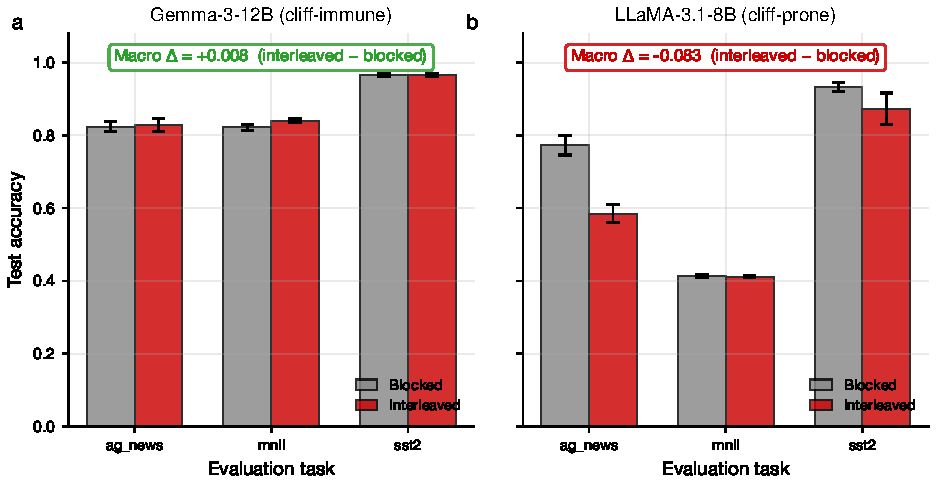
\includegraphics[width=0.8\textwidth]{revision/final_integration/si_order_final.pdf}
\caption{\textbf{\textcolor{blue}{Reported blocked/interleaved prompt comparison.}} \textcolor{blue}{Effects differ across
the illustrated models and conditions; this comparison does not establish invariance} to
order\textcolor{blue}{,} spacing \textcolor{blue}{or other} prompt \textcolor{blue}{arrangements}. Referenced as Supplementary Fig.~1 in the
main text.}
\label{sfig:ordering}
\end{figure}

\begin{figure}[h]
\centering
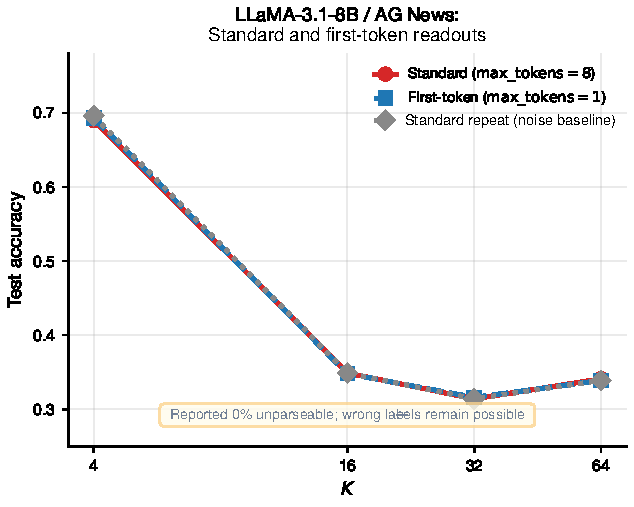
\includegraphics[width=0.8\textwidth]{revision/final_integration/si_readout_final.pdf}
\caption{\textbf{\textcolor{blue}{Standard and first-token readouts for the illustrated AG News curve.}}
The \textcolor{blue}{reported absence of unparseable labels addresses total parsing failure in this
comparison; it does not identify a} content\textcolor{blue}{-}integration \textcolor{blue}{mechanism or exclude label/recency
bias}. This is distinct from the \textcolor{blue}{entirely invalid} self-hosted \textcolor{blue}{cells} in Note~4\textcolor{blue}{.}}
\label{sfig:format}
\end{figure}

\begin{figure}[h]
\centering
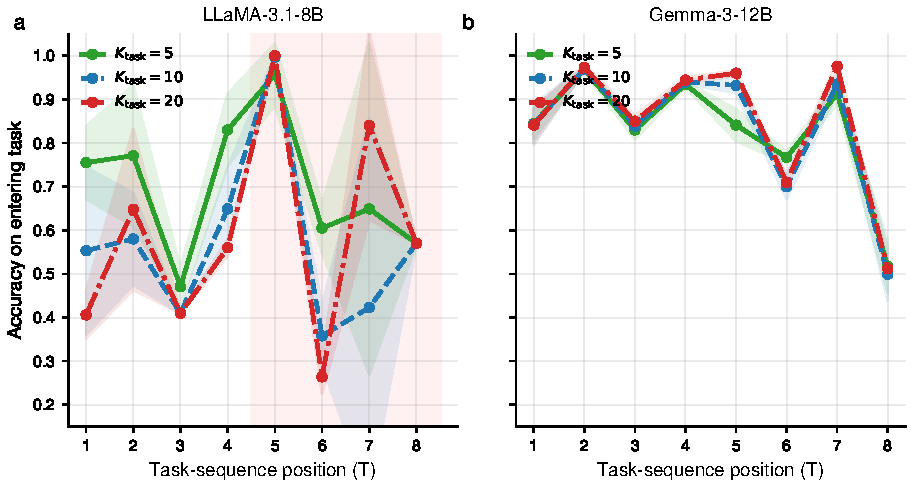
\includegraphics[width=0.8\textwidth]{revision/final_integration/si_task_sequence_final.pdf}
\caption{\textbf{\textcolor{blue}{Entering-task accuracy across a task sequence.}} \textcolor{blue}{The horizontal axis is
task-sequence position $T=1,\ldots,8$, not demonstrations per task. Lines use
$K_{\rm task}=5,10,20$ demonstrations per included task. The entering task changes with
position, so these curves do not isolate a fixed task's K-dependent cliff or a capacity
threshold.}}
\label{sfig:saturation}
\end{figure}

\begin{figure}[h]
\centering
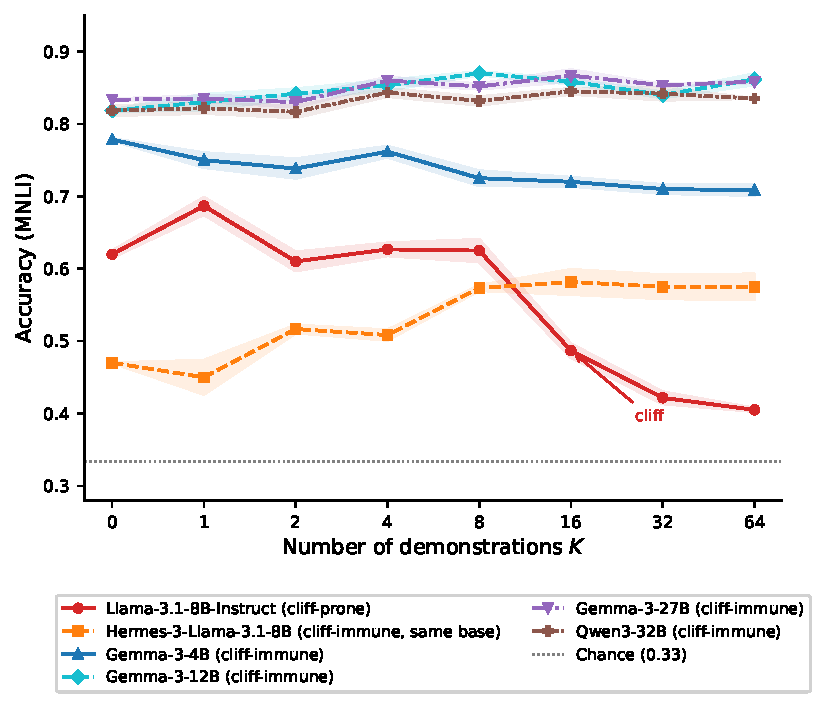
\includegraphics[width=0.85\textwidth]{figures/fig_ed_mnli_entailment.pdf}
\caption{\textbf{The regime split replicates on natural-language inference (MNLI).}
Three-class entailment, chance $=0.33$. Llama-3.1-8B-Instruct \textcolor{blue}{starts at $0.620$ at $K{=}0$,} peaks at $K{=}1$ ($0.687$)
and falls to $0.405$ by $K{=}64$, while Hermes-3-Llama-3.1-8B, which shares its base
checkpoint, rises from $0.470$ to $0.575$. Not every cliff-immune model gains on this task:
Gemma-3-4B declines from $0.778$ to $0.708$ across the sweep without approaching chance. \textcolor{blue}{Source-separated curves and denominator metadata are in \protect\path{revision/generated/mnli_absolute_curves.csv} and \protect\path{revision/generated/mnli_absolute_curve_summary.csv}.}}
\label{sfig:mnli}
\end{figure}

\begin{figure}[h]
\centering
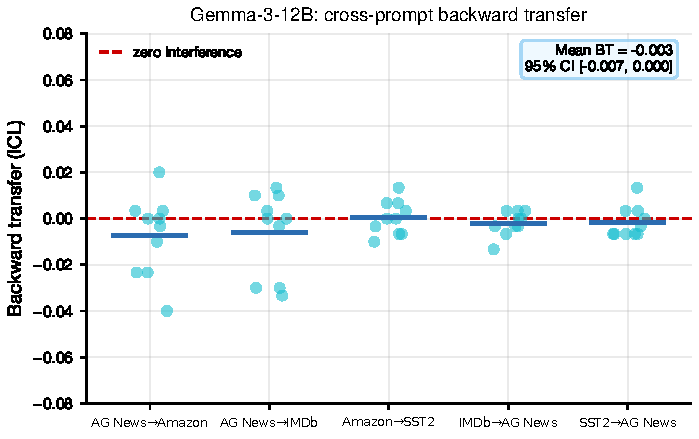
\includegraphics[width=0.66\textwidth]{figures/revision/si_cross_prompt_transfer_focused_v2.pdf}
\caption{\textbf{\textcolor{blue}{Reported cross-prompt backward transfer.}} \textcolor{blue}{Amazon denotes Amazon Electronics Sentiment. The illustrated Gemma-3-12B
summary is a consistency check (Note}~\textcolor{blue}{2), not evidence for a memory mechanism. Frozen,
stateless inference does not carry adaptation between independent prompts; the aggregate
results do not establish identical query/prompt identities for each reported comparison.}}
\label{sfig:stateless}
\end{figure}

\begin{figure}[h]
\centering
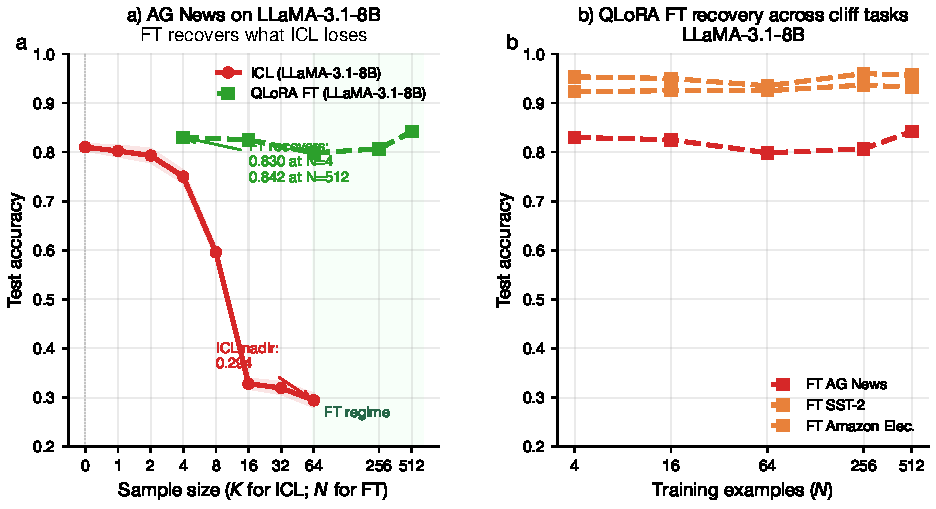
\includegraphics[width=0.8\textwidth]{figures/revision/si_ft_icl_comparison_focused.pdf}
\caption{\textbf{\textcolor{blue}{Reported fine-tuning and in-context accuracy.}} \textcolor{blue}{The illustrated comparison
motivates studying adaptation in weights; it does not establish permanent retention,
matched exposure/compute or the necessity of continual fine-tuning.}}
\label{sfig:ftrecovers}
\end{figure}

\begin{figure}[h]
\centering
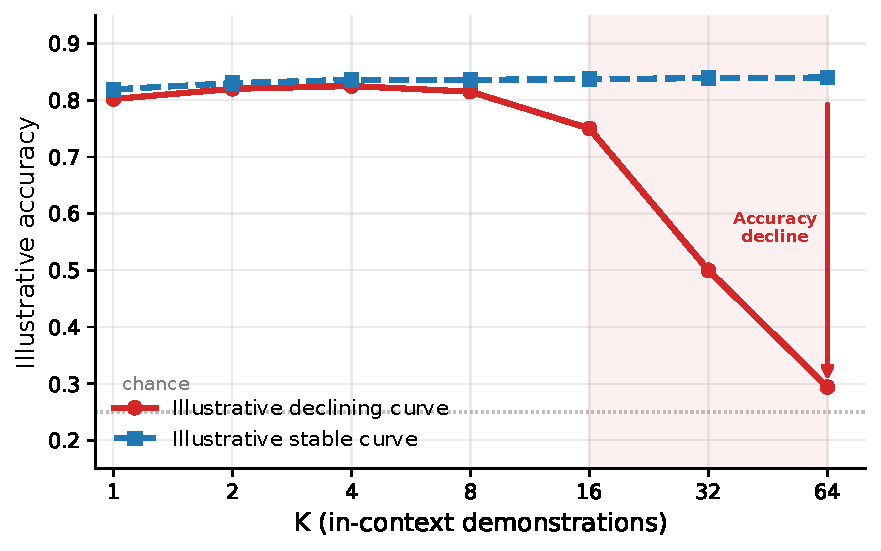
\includegraphics[width=0.92\textwidth]{figures/revision/si_context_curve_schematic_focused_v2.pdf}
\caption{\textbf{\textcolor{blue}{Schematic contrasting accuracy curves.}} \textcolor{blue}{The curves are illustrative,
not experimental measurements or a biological correspondence. CLS motivates a functional
comparison between rapid context use and adaptation in weights; this schematic does not
identify a bounded memory capacity or isolate a post-training recipe effect.}}
\label{sfig:concept}
\end{figure}

\end{document}
